\documentclass[10pt,a4paper]{article}
\usepackage{graphicx}
\graphicspath{ {figures/} }
\usepackage{amsmath}
\usepackage[utf8]{inputenc}
\usepackage{tikz}
\usepackage{float}
\usepackage{tabto}
\usepackage{caption}
\usepackage{subcaption}
\usetikzlibrary{shapes,snakes}
\usepackage{wrapfig}
\usepackage[hidelinks]{hyperref}
\usepackage{array}
\usepackage{xcolor}
\usepackage{xurl}

\usepackage[a4paper, total={6.5in, 8in}]{geometry}
\font\myfont=cmr12 at 30pt

\tikzstyle{arrow} = [thick,->,>=stealth]

\author{Ali El Hadi ISMAIL FAWAZ\\
\texttt{hadifawaz2291999@gmail.com}\\
\texttt{5460}\\\\
\and
LEBANESE UNIVERSITY - FACULTY OF ENGINEERING\\
BRANCH III\\\\
\small prepared for Dr. Youssef HARKOUS}

\date{\today}

\title{\myfont DIGITAL RECOGNITION}


\begin{document}

\maketitle
\titlepage
\tableofcontents
\newpage
\listoffigures
\newpage
\begin{center}
\section*{Acknowledgments}
First and foremost, we would like to thank the dean, the faculty director, the head of the electrical and telecommunication department and of course Dr. Y. Harkous for whom we are presenting our work.
\end{center}

\begin{abstract}
This paper presents the different ways of classifying the mnist digit recognition data set where we will compare the results of all the models used in this project.
\end{abstract}

\section{Introduction :}
\large “ The science and engineering of making intelligent machines, especially intelligent computer programs ”. -John McCarthy-\\
Humans are smart, but how does the human brain function, what happens when we try to learn,solve,think etc... Scientists created an approach called Artificial Intelligence (AI) to make a computer or a machine to behave just as humans, we can't know for sure if AI's methods are the same as the human mind's but we can know for sure that AI models these days can act like humans do, they can think, self learn, solve problems even humans couldn't solve them before or just not as fast as AI models. The aim of AI is to improve those skills that a human brain has. But unlike humans, AI needs algorithms and very specific guidance to achieve its goals because at the end of the day, it's still a machine.\\
We ask ourselves a simple question, how come AI hasn't taken over the world in every domain if it is that powerful? To answer this question we will study many methods in this project. Several techniques have been developed over the years to improve the results of AI models starting from simple machine learning algorithms to end up where we are today using deep learning techniques or what we call now neural networks, the name neural network is based on the idea of creating an artificial brain with artificial neurons. In this project we will discuss the simplest machine learning algorithm called Nearest Neighbor, small neural networks and large neural networks and compare there performance on image classification.

\section{Materials used :}
\large This project is a Graphical User Interface (GUI) application programmed in Python programming language so it would be friendly with users that don't have a lot of knowledge in programming, this GUI was built using a famous Python module called "Tkinter". Of course we can't study the performance of AI models without having a data set in out hands, so we will be using a very well known beginner data set called mnist digit recognition which contains a big number of images in black and white corresponding to handwritten digits from 0 to 9, the data set contains 70,000 28x28 gray scale images, each image has a label on it to indicate what digit is written in the image. For the machine learning and deep learning models we will be using 2 python modules "Keras" for deep learning and "tslearn" for the Nearest Neighbor algorithm.

\begin{figure}[H]
\centering
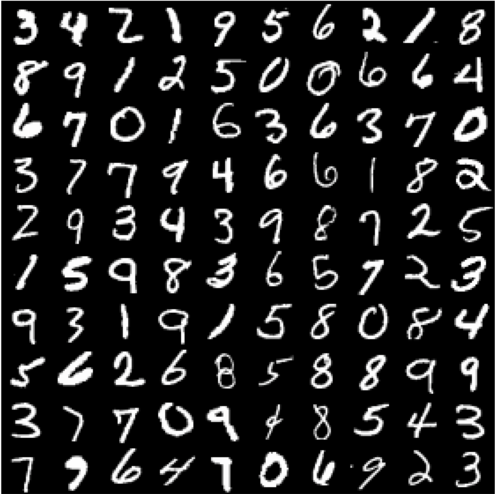
\includegraphics[scale=0.5]{mnist.png}\\
\caption{Examples of the mnist digit recognition data set}
\end{figure}
\begin{center}
\textcolor{blue}{\small\url {https://medium.com/@ankitbatra2202/mnist-handwritten-digit-recognition-with-pytorch-cce6a33cd1c1}}
\end{center}
\section{Data normalization :}
\large Data normalization is considered a very essential part of machine learning and deep learning, why is that? Before explaining why lets start by the definition of data normalization, normalizing a data set is to change in the numeric values of each attribute in the data set to a target scale. Note that not every data set requires a normalization , it is only required when the given features in a data set have different range of values, for example if we have a data set with two features : age (0-100) and income per month (0-20,000\$), we can see that the range of values in the income attribute is way bigger than the range of values in the age attribute so if we use an AI model without normalization it would take it a lot of time to learn from these values because they are too big like when calculating gradients (will discuss more in the next sections). Same thing applies to our digit recognition model because every pixel is an attribute and the range of values of each pixel is 0-255 so we may have a black pixel (0) and a white pixel (255) (remember we are dealing with a gray scale image so we have only 1 channel). There are many ways to normalize a data set, lets discuss about some of them:
\newpage
\subsection{Z-Normalization :}
This method of normalization consists of setting the mean of the attribute $x$ to 0 and the standard deviation of that attribute to 1 :\\\\
\begin{center}
$ x^{\prime} = \dfrac{x - \mu}{\sigma} $\\
\end{center}
where:
\begin{center}
$ \mu = \dfrac{1}{n}\sum_{i=1}^{i=n}x_i $
\end{center}
\begin{center}
$ \sigma = \sqrt{\dfrac{1}{n-1}\sum_{i=1}^{i=n}(x_i - \mu)^2} $
\end{center}

\subsection{Min-Max-Normalization :}
Thjs method changes the range of values of one attribute to [0,1] :\\
\begin{center}
$ x^{\prime} = \dfrac{x - \min{(x)}}{\max{(x)} - \min{(x)}} $
\end{center}

\subsection{Unit-Vector-Normalization :}
This method transforms the attribute vector to a unit vector ($ ||\vec{x}|| = 1 $) :\\
\begin{center}
$ \vec{x^{\prime}} = \dfrac{\vec{x}}{||\vec{x}||} $
\end{center}

\section{Train Test Split :}
In every AI model we need to split our data set into two new sets, first being the training set and second being the testing set. The AI model needs to self learn on the training self where it tries to learn the patterns of the data or tries to classify the instances etc... But while the model is training it being told by how much it is not learning correctly until it achieves its goal and have learned everything (will explain more in next sections). So why use the test set then? After our model have learned the data and knows what its work is, we need to evaluate it just like an exam for students, we teach students all semester and tell them what is right and wrong and correct there mistakes until we examine them in a test and evaluate there performance along the semester, same thing for AI models we need to evaluate its performance to see if it was learning well while the training was taking place.

\section{Nearest Neighbor :}
\large It is actually called K-Nearest-Neighbor (K-NN for short), where K being the number of the nearest neighbors of a vector. K-NN is one of the most basic algorithms used in classification problems, the idea behind it is to find the K nearest neighbors of a given instance from a whole data set so that this instance would belong to the class that has the most neighbors, for example if i am classifying an instance $ x $ with K=3 and we found those 3 nearest neighbors $ y_1,y_2,y_3 $, if $ y_1 $ and $ y_3 $ belong to class $ c_0 $ and $ y_2 $ belongs to class $ c_1 $ then $ x $ would be classified just like $ y_1 $ and $ y_3 $ (class $ c_0 $). In our project we considered K=1 so we only have to find one nearest neighbor and $ x $ would be classified like it. But how do we find the nearest neighbor? Based on what? That is where the math starts, to find the nearest neighbor we just have to calculate the distance of the vector $ x $ to all the instances in the data set and $ x $'s nearest neighbor would be the instance with the smallest distance from it, here are two methods to calculate the distance between two vectors that we used in this project :\\

\subsection{The Euclidean Distance (ED) :}
ED is the simple straight line distance between two points in a two dimensional plane (same applied in a N dimensional space) :\\

\begin{figure}[H]
\centering
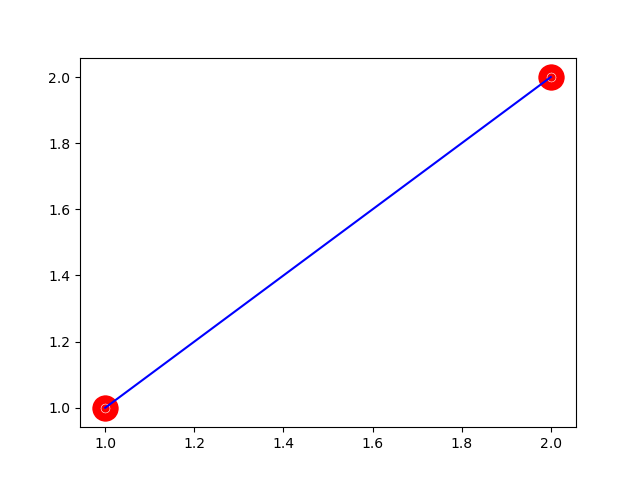
\includegraphics[scale=0.5]{ED.png}
\caption{Euclidean Distance between two points in a two dimensional plane.}
\end{figure}
\begin{center}
$ ED(x,y) = \sqrt{(x_1 - y_1)^2 + (x_2 - y_2)^2} $
\end{center}
This is if $ x $ and $ y $ are two points in a two dimensional plane, this how its calculated if x and y are n dimensional vectors:
\begin{center}
$ ED(x,y) = \sqrt{\sum_{i=1}^{i=n}(x_i - y_i)^2} $
\end{center}
\subsection{Dynamic Time Warping (DTW) :}
DTW is an algorithm to find the similarity between two time series, so first we have to define what is a time series.\\
A time series is sequence of data points equally spaced in time, for example if we want to log the income of a shop every 24 hours, then we would have as result a sequence of data points equally spaced by 24 hours which is a time series.
\begin{figure}[H]
\centering
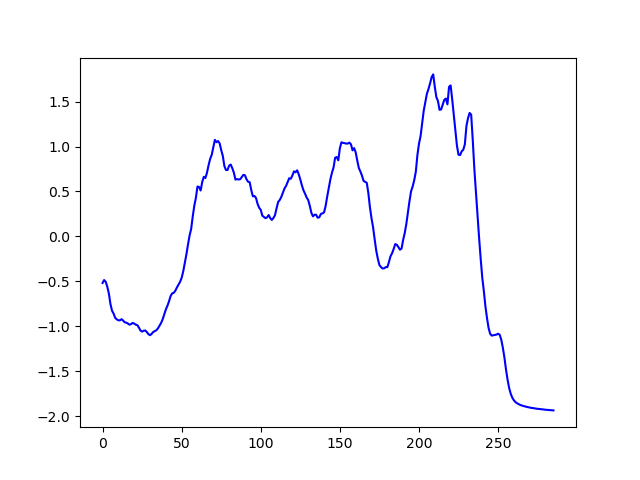
\includegraphics[scale=0.5]{Coffee.png}
\caption{Example of a Time Series, Coffee data set}
\end{figure}
\begin{center}
\textcolor{blue}{\small\url{https://www.cs.ucr.edu/~eamonn/time_series_data_2018/}}
\end{center}
So what is DTW? It is a method to find the optimal similarity between two time series, so eventually its a method to calculate the distance between two time series.\\
To explain more about DTW and how it works, lets consider these two time series:

\begin{center}
$ x = [5,3,4,0,1,3,5,0,2,1] $ and $ y = [11,12,11,8,9,11,12,9,11,10] $
\end{center}

So lets compare how the Euclidean Distance and Dynamic Time Warping distance are calculated between $ x $ and $ y $ :

In Figure \ref{fig:ED} we can see the two time series $ x $ (in blue) and $ y $ (in red), the green part of the plot represents the alignment between the two time series when we calculate the ED, so we align the data point from $ x $ at time $ t_i $ with the data point from $ y $ at time $ t_i $ also.\\
In Figure \ref{fig:DTW} we can see that the alignment is non-linear, instead it shows us the best alignment for a given data point from $ x $ with a specific data point from $ y $. As we can see that the data point from $ x $ at time $ t_0 $ is aligned with the data point from $ y $ at time $ t_1 $.

\begin{figure}[H]
\centering
\begin{subfigure}[b]{0.5\textwidth}
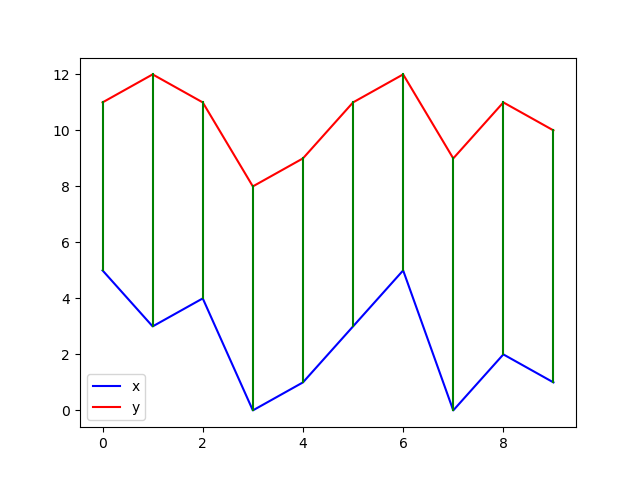
\includegraphics[scale=0.5]{ED_TS.png}
\caption{ED.}
\label{fig:ED}
\end{subfigure}
\begin{subfigure}[b]{0.45\textwidth}
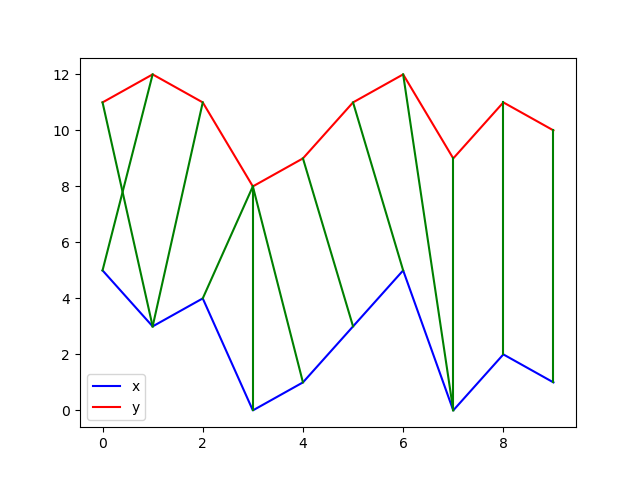
\includegraphics[scale=0.5]{DTW_TS.png}
\caption{DTW.}
\label{fig:DTW}
\end{subfigure}
\caption{Euclidean Distance alignment VS Dynamic Time Warping alignment.}
\label{fig:ED_DTW}
\end{figure}

So how to calculate this optimal distance between $ x $ and $ y $? We start by defining a two dimensional $ (n+1)*(m+1) $ matrix $ A $, $ n $ being the length of $ x $ and $ m $ the length of $ y $ ($ n $ can be different than $ m $). We then set $ A[0][0] = 0, A[0][1:m] = \infty $ and $ A[1:n][0] = \infty $.\\ For each cell of $ A $ we set :\\ $ cost = (x[i-1] - y[j-1])^2 $ and $ A[i][j] = cost + \min(A[i-1][j], A[i][j-1], A[i-1][j-1]) $, eventually the optimal DTW distance between $ x $ and $ y $ would be $ \sqrt{A[n][m]} $.

\section{Neural Networks (deep learning) :}
To define neural networks we have to know why were they called like that. Neural networks are a set of algorithms inspired by the functionality of the human brain, for example when we hear a sound, these sound waves are converted to brain waves signals to be processed but what we call the neurons in our brain, similarly this is the idea behind neural networks but of course we can not say that the algorithms we build are an explanation of how our brain studies information and learn new things, so we only took the nomenclature and called it neural networks and create artificial neuron networks (ANN's) to do the work.\\
So after this explanation above you would ask yourself, what do we mean by artificial neural networks? We can consider ANN's like a human brain, it needs to learn patterns from a given data, analyze the data, know how to classify the instance of a data, that data can be images, sounds etc... To go even deeper, ANN's are not more than learning an approximation of a function $ y = f(x) $, now what do we mean by approximation of a function? To answer this question lets start by the architecture of a neural network first, neural networks are made of layers, each layer has a functionality different than the others and a specific number of artificial neurons :
\subsection{Artificial Neurons :}
An artificial neuron can be defined as an input output system, where $ x $ is the input and $ y $ is the output, with a very simple linear relation between $ y $ and $ x $ (here $ x $ is one number not a vector):\\\\\\
\begin{figure}[H]
\centering
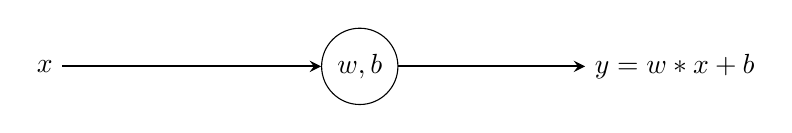
\begin{tikzpicture}

\node (x) at (-4,0) {$ x $};
\node (neuron) [draw,circle] at (0,0) {$ w,b $};
\node (y) at (4,0) {$ y = w*x + b $};
\draw [arrow] (x) -- (neuron);
\draw [arrow] (neuron) -- (y);
\end{tikzpicture}
\caption{Artificial Neuron.}
\end{figure}
Where $ w $ is called the weight and $ b $ the bias. The idea is that we have an input $ x $ and an output $ y $, we want to find the linear relation between $ x $ and $ y $ so eventually find the correct $ w $ and $ b $. How to do this? ANN's most important concepts are forward and backward propagation, in the forward propagation phase our goal is to calculate the output $ y^{\prime} = w*x ++ b $, backward propagation consists on calculating the loss between the real target $ y $ and the predicted target $ y^{\prime} $ and adjust the weight $ w $ and bias $ b $ and get closer to the correct values. How to adjust $ w $ and $ b $ and how to know when to stop? Our goal in ANN's is to minimize the loss as between $ y^{\prime} $ and $ y $ as much as possible and each time we calculate the loss (which should be decreasing from what we just explained) we adjust the weight and bias using a specific optimizer. Many optimizers are used these days, we are going to talk about a simple one called Gradient descent :
\subsection{Gradient Descent Optimizer :}
We explained before that after we calculate the loss we have to adjust the weight $ w $ and bias $ b $, lets consider that we calculated the loss $ L(y,y^{\prime}), y^{\prime} $ is a function of $ w $ and $ b $ and y is fixed to a given value that means $ L(y,y^{\prime}) $ is actually a function of $ w $ and $ b, L(w,b) $. So we adjust the weight and bias in this manner :\\
\begin{center}
$ w = w - \alpha*\dfrac{\partial L(w,b)}{\partial w} $ \hspace{1cm} and \hspace{1cm} $ b = b - \alpha*\dfrac{\partial L(w,b)}{\partial b} $
\end{center} 

Where $ \alpha $ is what we call the learning rate which is a hyper parameter, we mean by hyper parameter that it doesn't have a rule to be given a value because it depends on the data set and the functionality of the layer and the number of neurons etc... So the idea is we start with random values given for the weight and the bias, calculate $ y^{\prime} $, find the loss $ L(y,y^{\prime}) $, adjust $ w $ and $ b $ using the gradient descent explained above then keep doing the same work $ e $ times, where $ e $ is called the number epochs and in each epoch we perform the forward and backward propagation.\\
Lets see an example of what we just talked about :\\
\subsubsection{Linear Regression :}
Linear regression is a great example to explain the basics of deep learning (neural networks), lets consider having two variables : input $ x = 1 $ and output $ y = 2 $ and we want to find the linear relation between $ x $ and $ y $ (considering it exists), now we know this is a problem kids can solve but lets see how a neural network solves it. We will consider a network having only one neuron with weight $ w $ and bias $ b $ with initial values equal to 0 for both with a learning rate $ \alpha = 1 $ and we will use as a loss function :\\
\begin{center}
$ L(y,y^{\prime}) = |y^{\prime} - y| $\\
\end{center}
At epoch 1 :
\begin{center}
$ y^{\prime} = w*x + b = 0*1 + 0 = 0 $ \hspace{5mm} so \hspace{5mm} $ y^{\prime} - y = 0 - 2 = -2 $ \hspace{5mm} which is negative\\
So \hspace{5mm} $ L(y,y^{\prime}) = L(w,b) = y - y^{\prime} = y - w*x - b $ \hspace{5mm} to get :
\end{center}

\begin{center}
$ \dfrac{\partial L(w,b)}{\partial w} = -x = -1 $ \hspace{5mm} and \hspace{5mm} $ \dfrac{\partial L(w,b)}{\partial b} = -1 $
\end{center}
\begin{center}
So lets adjust $ w $ and $ b $ :\\
$ w = w - \alpha*\dfrac{\partial L(w,b)}{\partial w} = 0 - 1*(-1) = 1 $ \hspace{5mm} and \hspace{5mm} $ b = b - \alpha*\dfrac{\partial L(w,b)}{\partial b} = 0 - 1*(-1) = 1 $\\
Epoch 1 is done.
\end{center}

At epoch 2 :
\begin{center}
$ y^{\prime} = w*x + b = 1*1 + 1 = 1 + 1 = 2 $ \hspace{5mm} and \hspace{5mm} $ y = 2 $\\
So \hspace{5mm} $ L(w,b) = L(y,y^{\prime}) = |y^{\prime} - y| = |2 - 2| = 0 $\\
And with a loss being equal to zero, our work here is done and the correct values are $ w = 1 $ and $ b = 1 $ so we get the linear relation between input and output : $ y = w*x + b = x + 1 $
\begin{tikzpicture}
\draw (0,0) -- (10,0);
\end{tikzpicture}
\end{center}
Now what would happen if we have a vector of input values and a vector of output values instead but still only one neuron? In this case we will have to define a new hyper parameter called batch size, the idea behind this parameter is that we don't adjust the weight and bias after each value in the input vector begin forward propagated, but instead we find the mean of losses for each batch and adjust the weight and bias according to the mean of losses. To understand what was just explained lets consider having an input vector $ x $ of $ n $ values and an output vector $ y $ (of $ n $ values of course) and lets take an example of a batch size $ = 3 $, so what happens now is that the network will forward propagate each 3 values in the input vector and calculate the predicted output of each of them $ y^{\prime} $ then calculate the 3 losses for each of them and find there mean $ loss = \dfrac{1}{3}\sum_{i=1}^{i=3}L_i(y,y^{\prime}) $ then adjust one time $ w $ and $ b $ for these 3 batches using $ loss $ just calculated, this optimization is called Stochastic Gradient Descent(SGD).\\\\
Now if each value of the input vector is a vector it self of m values (input is a $ n*m $ matrix) but still one neuron, here $ w $ would be a vector of length $ m $ and $ b $ would still be one number, so to calculate the output of the neuron :\\
Lets consider $ m = 4 $ and that we are forward propagating the row $ i $ of the input matrix :\\
\begin{figure}[H]
\centering
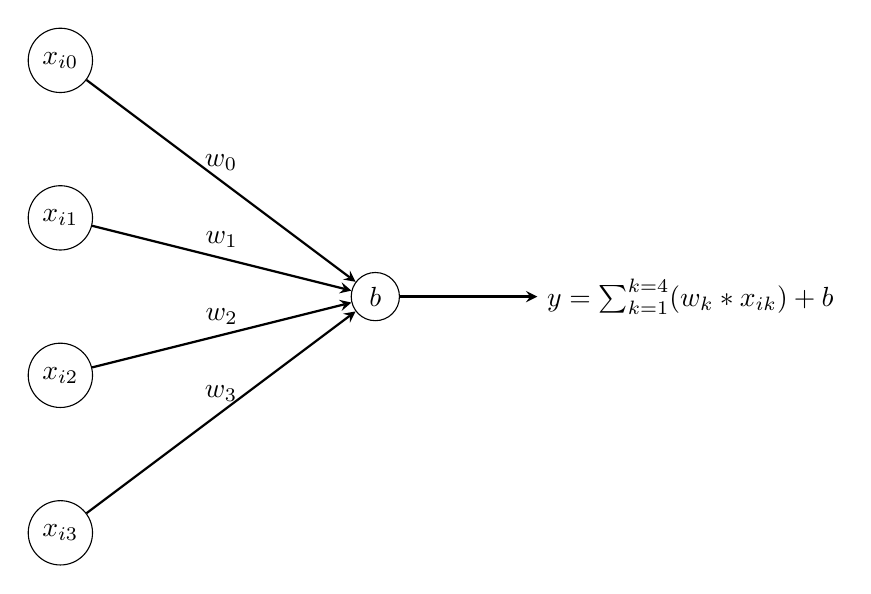
\begin{tikzpicture}

\node (x0) [draw,circle] at (-4,6) {$ x_{i0} $};
\node (x1) [draw,circle] at (-4,4) {$ x_{i1} $};
\node (x2) [draw,circle] at (-4,2) {$ x_{i2} $};
\node (x3) [draw,circle] at (-4,0) {$ x_{i3} $};
\node (neuron) [draw,circle] at (0,3) {$ b $};
\draw [arrow] (x0) -- node[anchor=south] {$ w_0 $} (neuron);
\draw [arrow] (x1) -- node[anchor=south] {$ w_1 $} (neuron);
\draw [arrow] (x2) -- node[anchor=south] {$ w_2 $} (neuron);
\draw [arrow] (x3) -- node[anchor=south] {$ w_3 $} (neuron);
\node (y) at (4,3) {$ y = \sum_{k=1}^{k=4}(w_k*x_{ik}) + b $};
\draw [arrow] (neuron) -- (y);

\end{tikzpicture}
\caption{One neuron with input vector of size $ m $.}
\end{figure}


In a more general way, consider having an input matrix $ X $ of $ n $ instances with each instance being a vector of $ m $ values (matrix $ X $ size $ n*m $), and $ u $ neurons in one layer, the output of that layer would be a vector of length $ u $, $ w $ would be a matrix of size $ (m*u) $ and $ b $ a vector of $ u $ values. To calculate the output vector of this layer :\\
\begin{center}
$ \vec{y^{\prime}} = w^{T}*\vec{x} + \vec{b} $
\end{center}

\subsection{Activation Functions :}
Till now we worked only with linearity between input and output, but what if it doesn't exist? Shouldn't we introduce some non-linearity to out neural network? Using what we call activation functions we can solve this problem, consider a layer of $ u $ neurons with an activation function $ f $, the work we explained before does not change, only that our output now would be $ f(output \hspace{2mm} explained \hspace{2mm} before) $. The activation function is also a hyper parameter which means there isn't a rule to choose one, several may be used like :
\subsubsection{Relu :}
\begin{center}
$ f(x) = max(0,x) $
\end{center}
\subsubsection{Hyperbolic tangent :}
\begin{center}
$ f(x) = \tanh(x) = \dfrac{2}{1 + e^{-2x}} - 1 $
\end{center}
\subsubsection{Sigmoid :}
\begin{center}
$ f(x) = \dfrac{1}{1 + e^{-x}} $
\end{center}
\begin{figure}[H]
\centering
\begin{subfigure}[b]{0.3\textwidth}
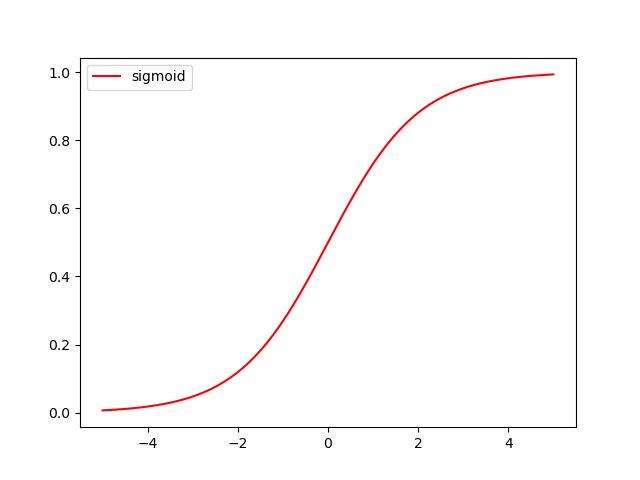
\includegraphics[scale=0.3]{sigmoid.png}
\caption{Sigmoid.}
\end{subfigure}
\begin{subfigure}[b]{0.3\textwidth}
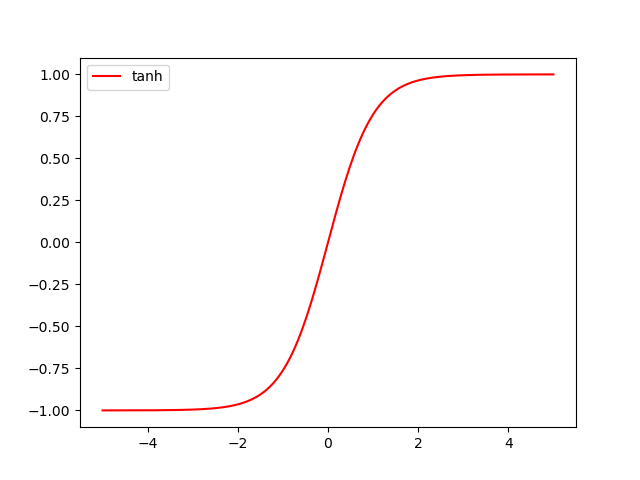
\includegraphics[scale=0.3]{tanh.png}
\caption{Tanh.}
\end{subfigure}
\begin{subfigure}[b]{0.3\textwidth}
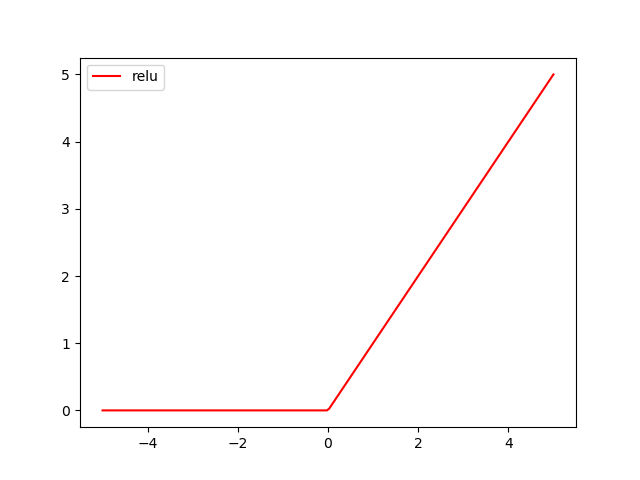
\includegraphics[scale=0.3]{relu.png}
\caption{Relu.}
\end{subfigure}
\caption{Examples of activation functions.}
\end{figure}
\subsubsection{Softmax :}
Every classification problem, when solved using neural networks must use a softmax activation function at the end of the network (last layer). If we had a given data set, we would have a test set and a training set for the ANN, when the ANN is being trained it should try to classify the training set's instances and see how much its prediction was accurate by calculating the loss between the real target and predicted target, but how does softmax helps predict to which class an instance belongs? Lets consider an ANN with $ n $ layers, where the $ n^{th} $ layer apply the softmax function, so the input of the last layer is the output of the $ (n-1)^{th} $ layer, if $ x $ is the input of the last layer of length $ m $ and $ y $ its output of length $ k $ then :\\
We calculate the output of the last layer $ u $ before applying the softmax function
\begin{center}
$ \vec{u} = w^{T}*\vec{x} + \vec{b} $\\
$ w $ being the weights matrix of the last layer and $ \vec{b} $ its bias vector.
\end{center}

So:
\begin{center}
$ y_i = \dfrac{e^{u_i}}{\sum_{j=0}^{j=k}e^{u_j}} $
\end{center}
And that produces the probability of the instance of being classified in any of the $ k $ classes we have, so that is a vector of probabilities and how can we calculate the loss given that the real target is only one number? To solve this problem we transform the real targets we have (vector of targets, each target is a class) to a binary matrix, for example if we had a vector of real targets $ [0,1,2,2] $ that means we only have three classes here 0, 1 and 2 then we would transform it to :\\\\
$\begin{pmatrix}
1 & 0 & 0\\
0 & 1 & 0\\
0 & 0 & 1\\
0 & 0 & 1
\end{pmatrix}$\\\\
This way we can calculate the loss between each row of that matrix and the probability vector given by the softmax layer, but here we use the Categorical Cross-Entropy (CCE) loss :\\
\begin{center}
$ CCE = -\sum_{i=0}^{i=C}y_i*\log(y^{\prime}_i) $
\end{center}
\begin{center}
$ C $ being the number of classes, $ y $ the vector target (a row from the matrix shown above) and $ y^{\prime} $ the output of the softmax layer.
\end{center}
\subsection{Layers :}
There is a lot of layers that we can explain in deep learning so we're going to stick with the ones we used in our project. A layer in ANN is a container of neurons, it holds a collection of neurons that performs the same function and the same activation function to provide a specific output :
\subsubsection{Input Layer :}
Every neural network must have an input layer, its job is to receive the input data from web service or a csv file etc...
\subsubsection{Output Layer :}
Also every neural network must have an output layer, it is responsible for producing the final results of the network like the layer with the softmax activation function explained before.
\subsubsection{Hidden Layer :}
Hidden layers reside in between the input and output layers, they are not visible to the external system, there could be 0 or more hidden layers in an ANN. There is a lot of types of hidden layers so we are going to explain the ones we used in our project :
\paragraph{6.4.3.1 Dense Layer :}
The dense layer was explained before, it consists of having $ u $ neurons and one activation function $ f $ and its output (lets call it $ y $) is calculated in the following way :\\
\begin{center}
$ \vec{y} = f(w^{T}*\vec{x} + \vec{b}) $
\end{center}
The number of weights in the matrix $ w $ is $ n*u $ where $ n $ is the length of the input to this layer and the number of biases used is $ u $.\\
So in total $ n*u + u $ parameters are used in a dense layer.
\paragraph{6.4.3.2 Max Pooling 2D :}
The goal of a max pooling layer is to just reduce the size of the input, lets say you have a $ 4x4 $ matrix :\\\\
$D = 
\begin{pmatrix}
1 & 3 & 2 & 1\\
2 & 9 & 1 & 1\\
1 & 3 & 2 & 3\\
5 & 6 & 1 & 2
\end{pmatrix}
$
Then applying a $ (2,2) $ max pooling on it would produce :
$D^{\prime} = 
\begin{pmatrix}
9 & 2\\
6 & 3
\end{pmatrix}
$\\\\
As you can see the size has been divided by 2 on width and height, because we applied a $ (2,2) $ filter where each of the $ 4 (2,2) $ sub matrix is replaced by the maximum of its values, so the filter would jump 2 steps vertically and horizontally.
\paragraph{6.4.3.3 2D Convolution Layer (Conv2D) :}
Same way we used a 2 dimensional filter in the max pooling layer we are going to use one here, but the difference is that this time the filter jumps 1 step (regardless of its size) vertically and horizontally. To understand how the filter works lets see an example :\\
Lets consider having the same matrix we used in the previous section about max pooling layer, we will use this matrix as a $ (2,2) $ filter :\\\\
$F = 
\begin{pmatrix}
1 & -1\\
-1 & 1
\end{pmatrix}
$
The first sub matrix the filter sees is : 
$A = 
\begin{pmatrix}
1 & 3\\
2 & 9
\end{pmatrix}
$\\\\
So to calculate the after filtering results we compute this :\\
\begin{center}
$ B = \sum_{i=1}^{i=2}F_i*A_i $
\end{center}
\newpage
And we keep moving the filter around till we get a new matrix, for the above example the after filtering results would be :\\\\
$D^{\prime} = 
\begin{pmatrix}
5 & -7 & -1\\
-5 & -9 & 1\\
-1 & -4 & 0
\end{pmatrix}
$
A convolution layer creates many filters and does the same work\\\\for each one of them, using convolution layers the ANN can learn certain patterns in the data for example vertical or horizontal lines or the edges in a given image.
\paragraph{6.4.3.4 Dropout Layer :}
A dropout layer has only one parameter which is a probability $ p $ called keep probability, from its name it seems like something is going to get dropped out and some are going to stay. Lets say we have 2 hidden layers, the first containing $ n $ neurons and the second $ m $ neurons, we know that the input of the second one is the output of the first one, so if we place a dropout layer between them with a keep probability $ p = 0.4 $ then $ 60\% $ of the neurons of the first layer will be zero out so they won't affect as inputs to the second layer and $ 40\% $ of those neurons only pass to the second layer, of course the choice of the dropped neurons is equally probable.
\begin{figure}[H]
\centering
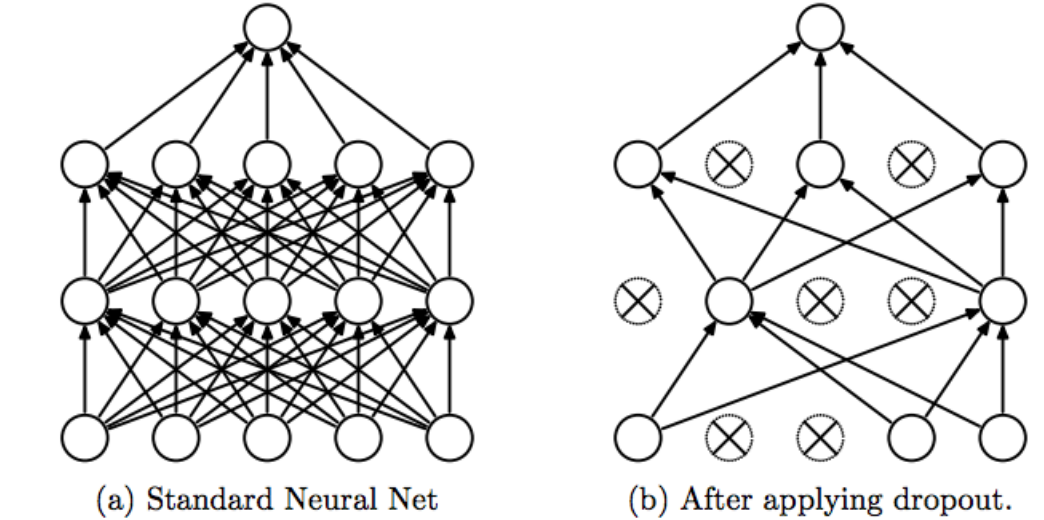
\includegraphics[scale=0.4]{dropout.png}
\caption{Visualization of a network with dropout.}
\end{figure}
\begin{center}
\textcolor{blue}{\small rivastava, Nitish, et al. ”Dropout: a simple way to prevent neural networks from
overfitting”, JMLR 2014}
\end{center}
\paragraph{6.4.3.5 Flatten Layer :}
This layer does not have any parameters and it just takes the output of a hidden layer or input layer and transforms its data to a 1 dimensional vector.

\section{Putting It All Together :}

You can find the code of our project \textcolor{blue}{\href{https://github.com/hadifawaz1999/Mini_Project}{here}.}

Our project is a simple Graphical User Interface (GUI) created in python using the Tkinter module where the user can choose any of the 3 methods we talked about (NN-ED, NN-DTW, ANN) to test the model's classification. For all of the 3 methods we talked about we gathered some results, for the nearest neighbor algorithm (using ED and DTW) we did only one trial with only 200 samples of the train set and 100 samples of the test set because nearest neighbor with ED is a O(n) algorithm and DTW is a O(n*m) algorithm so with 60,000 train samples and 1000 test samples it would take a lot of time for the algorithm to finish even with the optimized functions that we used from Tslearn and Sklearn modules that we used to evaluate the algorithms. For the neural networks we implemented our model using the Keras module with 9 different approaches so we can compare the results and choose the best model, because the number of hyper parameters that a neural network has is very large so we had 3 different optimizers : SGD, Adam and Adadelta, 2 different learning rates : 0.01 and 0.001 and 2 different batch sizes : 128 and 512 but with a fixed number of epochs equal to 10.\\\\
Note : For the neural network method we used the whole data set.\\
Our Neural Network has the following architecture :\\
\begin{itemize}
\item Layer 1 : Input layer
\item Layer 2 : Conv2D layer, number of filters is 32 and kernel size is (3,3), relu activation function
\item Layer 3 : Conv2D layer, number of filters is 64 and kernel size is (3,3), relu activation function
\item Layer 4 : MaxPool2D layer, pool size is (2,2)
\item Layer 5 : Dropout layer, with a keep probability of 25\%
\item Layer 6 : Flatten layer
\item Layer 7 : Dense layer, number of units is 128 with a relu activation function
\item Layer 8 : Dropout layer, with a keep probability of 50\%
\item Layer 9 : Output Dense layer, number of units is 10 given the number of digits we have with a softmax activation function
\end{itemize}

\section{Results :}
Here is a table of the results we got for the Neural Networks method :\\\\

\begin{center}
\begin{tabular}{|p{3cm}||p{3cm}|p{3cm}|p{3cm}|p{3cm}|}
\hline
\multicolumn{5}{|c|}{Neural Network Results} \\
\hline
Optimizer & Batch Size & Learning Rate & Number of Epochs & Test Accuracy\\
\hline
SGD & 128 & 0.01 & 10 & 96.42\%\\
\hline
SGD & 128 & 0.001 & 10 & 91.92\%\\
\hline
SGD & 512 & 0.01 & 10 & 94.21\%\\
\hline
Adam & 128 & 0.01 & 10 & 98.72\%\\
\hline
Adam & 128 & 0.001 & 10 & 99.02\%\\
\hline
Adam & 512 & 0.01 & 10 & 98.81\%\\
\hline
Adadelta & 128 & 0.01 &10 & 93.63\%\\
\hline
Adadelta & 128 & 0.001 &10 & 81.55\%\\
\hline
Adadelta & 512 & 0.01 &10 & 91.15\%\\
\hline
\end{tabular}
\end{center}

Here is a table of the results we got for the nearest neighbor method :\\\\

\begin{center}
\begin{tabular}{|p{5cm}||p{3cm}|p{3cm}|p{3cm}|}
\hline
\multicolumn{4}{|c|}{Nearest Neighbor Results}\\
\hline
Distance & Train set size & Test set size & Test accuracy\\
\hline
Euclidean & 200 & 100 & 75\%\\
\hline
Dynamic Time Warping & 200 & 100 & 83\%\\
\hline
\end{tabular}
\end{center}

\section{Discussion}

We can observe from our results using Nearest Neighbor that this method is not very efficient though of course using DTW is way better than using ED because DTW finds the optimal alignment between the two samples but its problem is the time complexity, if the samples are of length $ n $ and $ m $ than the algorithm would have a time complexity of $ O( n*m ) $.\\\\\\
On the other hand we can see that the best way was to use neural networks, especially when using convolution layers because it can detects very specific patterns in the image. Although that using the optimizer Adam gave the best test accuracy, we can't say that its the best optimizer there is for all the neural networks we can build even the learning rate and the batch size because it always depends on the data set and on the architecture of a neural network.\\
But we can observe from our results that for that specific architecture that we built and the given data set, the best way is to use Adam optimizer with a learning rate of 0.001, batch size equal to 128 and repeat the work 10 times (number of epochs) but that doesn't mean that there isn't even better ways because in the end this is a research based project that we worked on.

\section{Conclusion}

After all we explained and observed in our little research we can say at the end that the best way to create an Artificial Intelligence machine is to use neural networks (for now at least), but more importantly, when dealing with neural networks we always have what we called before hyper parameters, the number of these parameters can be very large because we have to choose what are the number of layers and there types, what is the activation function for each layer and the parameters of each layer, the learning rate and batch size etc...\\
But eventually the neural network could learn and teach itself how to classify these images just like a human can do, the teaching phase was way slower than how humans can learn but it classified 10,000 images in seconds which takes a human a lot longer than that obviously.\\\\
So no matter what our data set is and what architecture we build, we always need to make trials to see and compare results to eventually choose the best method and of course learn why is this better than before. But the community asks always the same question : Can we trust AI ? This question opens a new kind of research called XAI : Explainable Artificial Intelligence, because we need to make the community to believe that AI can be trustworthy because in the end it is what would take over everything in the future.

\section{References :}

\begin{itemize}

\item \textcolor{blue}{\url{https://becominghuman.ai/introduction-to-artificial-intelligence-5fba0148ec99}}
\item \textcolor{blue}{\url{https://www.overleaf.com/learn/latex}}
\item \textcolor{blue}{\url{https://medium.com/@urvashilluniya/why-data-normalization-is-necessary-for-machine-learning-models-681b65a05029}}
\item \textcolor{blue}{\url{https://towardsdatascience.com/understand-data-normalization-in-machine-learning-8ff3062101f0}}
\item \textcolor{blue}{\url{https://medium.com/datadriveninvestor/k-nearest-neighbors-knn-7b4bd0128da7}}
\item \textcolor{blue}{\url{https://medium.com/@srishtisawla/k-nearest-neighbors-f77f6ee6b7f5}}
\item \textcolor{blue}{\url{https://medium.com/datadriveninvestor/dynamic-time-warping-dtw-d51d1a1e4afc}}
\item \textcolor{blue}{\url{https://towardsdatascience.com/dynamic-time-warping-3933f25fcdd}}
\item \textcolor{blue}{\url{https://medium.com/@purnasaigudikandula/a-beginner-intro-to-neural-networks-543267bda3c8}}
\item \textcolor{blue}{\url{https://mathanrajsharma.medium.com/softmax-activation-function-e582ea53ada7}}
\item \textcolor{blue}{\url{https://medium.com/fintechexplained/neural-network-layers-75e48d71f392}}
\item \textcolor{blue}{\url{https://gombru.github.io/2018/05/23/cross_entropy_loss/}}
\item \textcolor{blue}{\url{https://medium.com/datathings/dense-layers-explained-in-a-simple-way-62fe1db0ed75}}
\item \textcolor{blue}{\url{https://medium.com/@brightonnkomo/convolutional-neural-networks-part-4-the-pooling-and-fully-connected-layer-394ec01fb00d}}
\item \textcolor{blue}{\url{https://xzz201920.medium.com/conv1d-conv2d-and-conv3d-8a59182c4d6}}
\item \textcolor{blue}{\url{https://medium.com/@amarbudhiraja/https-medium-com-amarbudhiraja-learning-less-to-learn-better-dropout-in-deep-machine-learning-74334da4bfc5}}
\item \textcolor{blue}{\url{https://towardsdatascience.com/the-most-intuitive-and-easiest-guide-for-convolutional-neural-network-3607be47480}}
\item \textcolor{blue}{\url{https://keras.io/}}
\item \textcolor{blue}{\url{https://scikit-learn.org/stable/}}
\item \textcolor{blue}{\url{https://tslearn.readthedocs.io/en/stable/}}
\item \textcolor{blue}{\url{https://numpy.org/}}
\item \textcolor{blue}{\url{https://matplotlib.org/}}
\item \textcolor{blue}{\url{https://docs.python.org/3/library/tkinter.html}}
\item \textcolor{blue}{\url{https://docs.python.org/3/}}

\end{itemize}

\end{document}